%% 01-basics.tex — Codechella Madrid 2026: Foundations of DiD (90 minutes)
%% Scott Cunningham, CUNEF, May 25--28, 2026
%%
%% Compile: pdflatex 01-basics.tex
%% Style:   remix.sty (in same directory)

\documentclass[aspectratio=169,11pt]{beamer}
\usepackage{remix}

%% ===========================================================
%% MADRID PALETTE — Sunset on Gran Vía
%% Replaces the Glasgow green scheme with warm terracotta + twilight navy
%% ===========================================================
\definecolor{madridterracotta}{HTML}{C44536}  % Primary accent — Iberian terracotta
\definecolor{madridtwilight}{HTML}{2C3E5C}    % Section headers — twilight sky navy
\definecolor{madridpeach}{HTML}{FBE5D0}       % Tints, alert blocks — sunset peach
\definecolor{madridgold}{HTML}{C9982A}        % Secondary accent — Spanish gold
\definecolor{madridcream}{HTML}{FAF6EE}       % Background — warm cream
%% Remap remix.sty's green-based palette to Madrid colors
\colorlet{remixgreen}{madridterracotta}
\colorlet{remixgreendark}{madridtwilight}
\colorlet{remixgreenlight}{madridpeach}
\colorlet{forest}{madridgold}
\colorlet{accent}{madridterracotta}
\colorlet{accentdark}{madridtwilight}
\colorlet{cream}{madridcream}
%% Refresh beamer color templates that were locked at load time
\setbeamercolor{structure}{fg=accent}
\setbeamercolor{alerted text}{fg=accent}
\setbeamercolor{itemize item}{fg=accent}
\setbeamercolor{itemize subitem}{fg=accent}
\setbeamercolor{enumerate item}{fg=accent}
\setbeamercolor{enumerate subitem}{fg=accent}
\setbeamercolor{block title alerted}{fg=charcoal,bg=remixgreenlight}
\setbeamercolor{block body alerted}{fg=slate,bg=remixgreenlight}

\usepackage{tikz}
\usetikzlibrary{positioning,arrows.meta,calc,shapes.geometric,fit,backgrounds}
\usepackage{listings}
\usepackage{xcolor}
\usepackage{booktabs}
\usepackage{colortbl}

%% ---------- Sandwich-estimator color tracing (bread / meat) ----------
\definecolor{breadcolor}{HTML}{2B6CB0}
\definecolor{meatcolor}{HTML}{A51C30}
\newcommand{\bread}[1]{\textcolor{breadcolor}{#1}}
\newcommand{\meat}[1]{\textcolor{meatcolor}{#1}}

%% ---------- TikZ styles in the PREAMBLE ----------
\tikzset{
  ingredient/.style={
    rectangle, rounded corners=2pt, draw=accent, line width=0.8pt,
    fill=cream, text=charcoal, font=\bfseries,
    minimum width=4.8cm, minimum height=1.6cm, align=center
  },
  ingredientdone/.style={
    rectangle, rounded corners=2pt, draw=accent, line width=0.8pt,
    fill=remixgreenlight, text=charcoal, font=\bfseries,
    minimum width=4.8cm, minimum height=1.6cm, align=center
  },
  ingredientpending/.style={
    rectangle, rounded corners=2pt, draw=warmgray, line width=0.6pt, dashed,
    fill=white, text=warmgray, font=\bfseries,
    minimum width=4.8cm, minimum height=1.6cm, align=center
  },
  cell/.style={
    rectangle, draw=charcoal, line width=0.5pt,
    fill=lightbg, text=charcoal,
    minimum width=3.0cm, minimum height=1.3cm, align=center, font=\small
  },
  celltreated/.style={
    rectangle, draw=accent, line width=1.2pt,
    fill=remixgreenlight, text=charcoal,
    minimum width=3.0cm, minimum height=1.3cm, align=center, font=\small
  },
  conceptbox/.style={
    rectangle, rounded corners=3pt, draw=#1, line width=0.8pt,
    fill=white, text=charcoal, font=\small,
    minimum width=5.2cm, minimum height=2.6cm, align=left,
    text width=4.8cm, inner sep=8pt
  },
  trendline/.style={line width=1pt, accent},
  trendcontrol/.style={line width=1pt, slate, dashed},
}

%% ---------- listings setup ----------
\lstset{
  basicstyle=\ttfamily\footnotesize,
  keywordstyle=\color{accentdark}\bfseries,
  commentstyle=\color{warmgray}\itshape,
  stringstyle=\color{ocean},
  backgroundcolor=\color{lightbg},
  frame=single,
  framesep=4pt,
  rulecolor=\color{warmgray!40},
  columns=fullflexible,
  showstringspaces=false,
  breaklines=true,
  numbers=none,
  xleftmargin=0.4em,
  xrightmargin=0.4em,
}

%% Footer + section divider venue
\renewcommand{\remixfooter}{Codechella Madrid 2026\,\textperiodcentered\,CUNEF\,\textperiodcentered\,May 25--28}
\renewcommand{\remixsectionvenue}{Codechella Madrid \textperiodcentered\ May 2026}

\begin{document}

%% ===========================================================
%% TITLE — Madrid banner override of \remixtitleframe
%% Uses codechella_2026.jpg as a top banner; title text below.
%% ===========================================================
\begingroup
\setbeamertemplate{footline}{}
\begin{frame}[plain]
  \begin{tikzpicture}[remember picture,overlay]
    %% Cream background
    \fill[cream] (current page.south west) rectangle (current page.north east);
    %% Banner: Madrid skyline at the top, full width.
    %% Clipped to top 55% of slide so the photo doesn't bleed into the title text.
    \begin{scope}
      \clip (current page.north west) rectangle ([yshift=-0.55\paperheight]current page.north east);
      \node[anchor=north,inner sep=0pt] at (current page.north) {%
        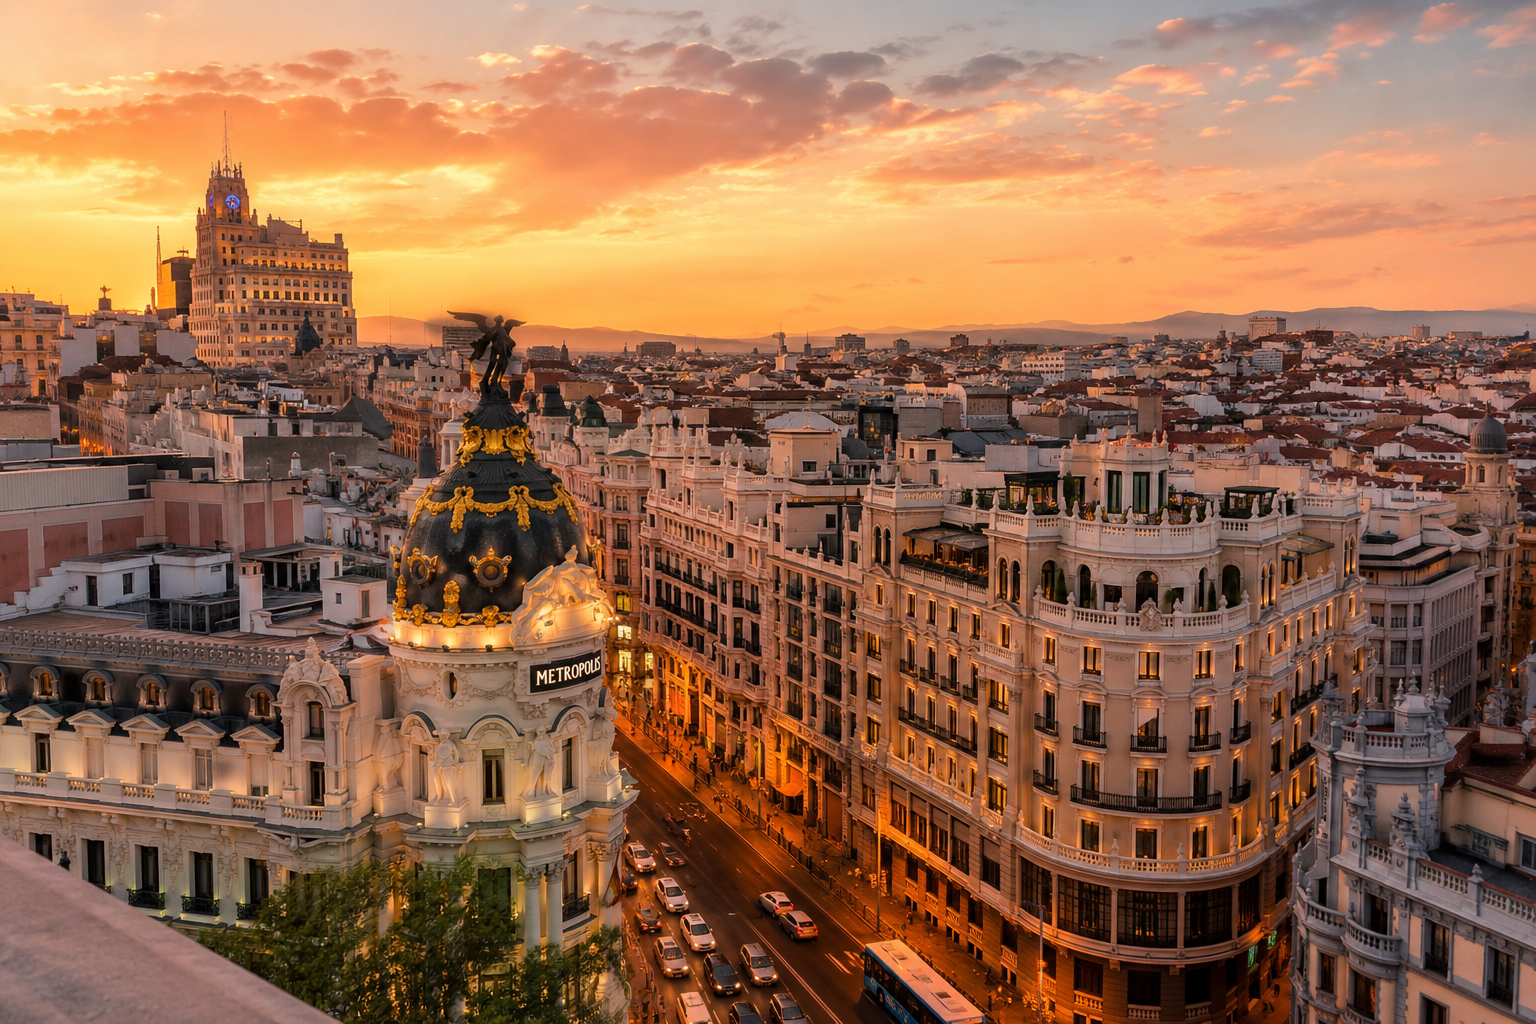
\includegraphics[width=\paperwidth]{codechella_2026.jpg}%
      };
    \end{scope}
    %% Thin accent rule below the banner
    \draw[accent,line width=1pt]
      ([yshift=-0.555\paperheight]current page.north west) --
      ([yshift=-0.555\paperheight]current page.north east);
    %% Title block in the lower zone
    \node[anchor=north,text width=0.85\paperwidth,align=center] at ([yshift=-0.575\paperheight]current page.north) {%
      {\color{accent}\fontsize{9pt}{11pt}\selectfont\bfseries\MakeUppercase{Codechella Madrid 2026}\par}%
      \vspace{0.3em}
      {\color{charcoal}\bfseries\fontsize{20pt}{24pt}\selectfont Foundations of Difference-in-Differences\par}%
      \vspace{0.25em}
      {\color{warmgray}\itshape\fontsize{12pt}{14pt}\selectfont Day 1: The 2$\times$2, Parallel Trends, and Event Studies\par}%
      \vspace{0.8em}
      {\color{charcoal}\fontsize{10.5pt}{13pt}\selectfont Scott Cunningham \textperiodcentered\ Baylor University\par}%
      \vspace{0.1em}
      {\color{warmgray}\fontsize{9.5pt}{12pt}\selectfont CUNEF Auditorium \textperiodcentered\ May 25--28, 2026\par}%
    };
  \end{tikzpicture}
\end{frame}
\endgroup

%% ===========================================================
%% HOUSEKEEPING — opening slides (welcome, team, mission, schedule, today, week)
%% One idea per slide. No walls of text.
%% ===========================================================

%% --- H.1 Welcome ---
\begin{frame}{Welcome to Codechella Madrid 2026}
\vspace{2.5em}
\begin{center}
{\Large Our third annual workshop here at CUNEF.}
\end{center}
\end{frame}

%% --- H.2 The team ---
\begin{frame}{Mixtape Sessions}
\vspace{1.6em}
\begin{center}
{\Large \textbf{Scott Cunningham} \;\textperiodcentered\; Baylor}\\[0.6em]
{\Large \textbf{Kyle Butts} \;\textperiodcentered\; Arkansas}\\[0.3em]
{\small\color{warmgray}\itshape (at home with his new baby!)}\\[1.2em]
{\large with \textbf{Mark Anderson} \;(Montana State)}\\[0.3em]
{\large \textbf{Dan Rees} \;(UC3M) \;\textperiodcentered\; \textbf{Agust\'in Casas} \;(CUNEF)}
\end{center}
\end{frame}

%% --- H.3 The mission ---
\begin{frame}{What we're here for}
\vspace{2.5em}
\begin{center}
{\Large Practical causal inference.}\\[1.2em]
{\large The methods.}\\[0.6em]
{\large Using them well.}\\[0.6em]
{\large Our opinions, along the way.}
\end{center}
\end{frame}

%% --- H.4 The week ---
\begin{frame}{The week}
\vspace{0.15em}
\begin{center}
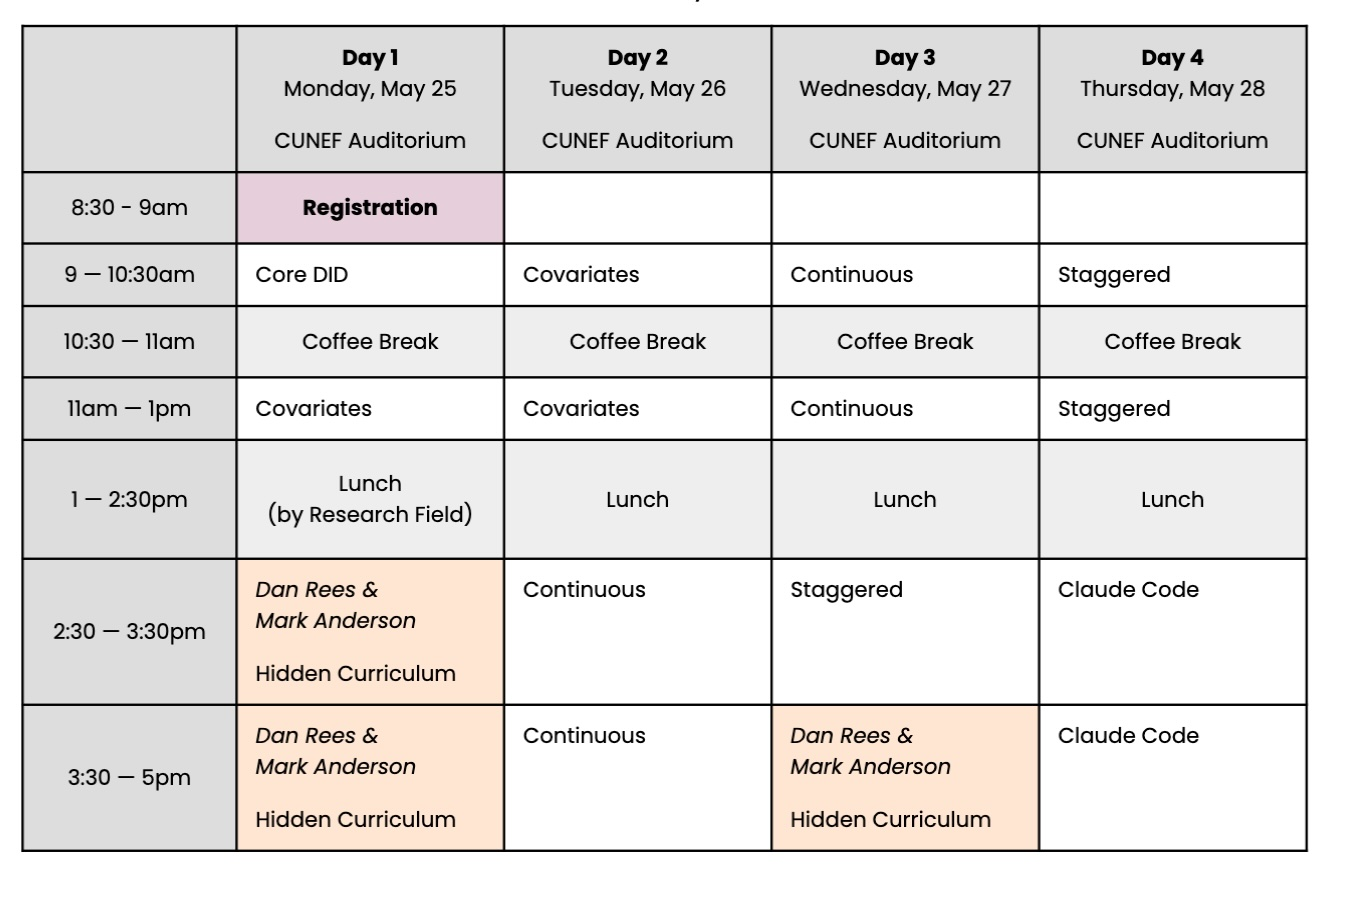
\includegraphics[width=0.86\textwidth,height=0.82\textheight,keepaspectratio]{figures/codechella_schedule_2026.jpg}
\end{center}
\end{frame}

%% --- H.5 Today's focus ---
\begin{frame}{Today: the basics of DiD}
\vspace{1.4em}
\begin{center}
{\Large Four moving parts.}\\[1.8em]
{\large \highlight{Calculation.}}\\[0.5em]
{\large \highlight{Identification.}}\\[0.5em]
{\large \highlight{Regressions.}}\\[0.5em]
{\large \highlight{Falsifications.}}
\end{center}
\end{frame}

%% --- H.6 The rest of the week ---
\begin{frame}{After today}
\vspace{1.4em}
\begin{center}
\large
\begin{tabular}{@{}rl@{}}
\textbf{Covariates} & \textperiodcentered\; Mon PM + all of Tue \\[0.5em]
\textbf{Continuous DiD} & \textperiodcentered\; Tue PM + Wed AM \\[0.5em]
\textbf{Staggered DiD} & \textperiodcentered\; Wed PM + Thu AM \\[0.5em]
\textbf{Hidden Curriculum} & \textperiodcentered\; Mon \& Wed afternoons, with Mark \& Dan \\[0.5em]
\textbf{Claude Code} & \textperiodcentered\; Thu PM \\
\end{tabular}
\end{center}
\end{frame}

%% ===========================================================
%% SECTION 1. DiD's empirical roots
%% ===========================================================
\remixsection{1.\ DiD's Empirical Roots}

%% --- 1.1 Semmelweis ---
\begin{frame}{Vienna, 1840s: two clinics, two mortality rates}
\vspace{0.4em}
\begin{itemize}
  \item Vienna General Hospital, First Obstetric Clinic
  \item Pregnant women were assigned to the \textit{physicians' wing} or the \textit{midwives' wing} by day of admission --- effectively at random
  \item Physicians' wing: \highlight{13--18\% mortality} from puerperal fever
  \item Midwives' wing: \highlight{about 3\%}
  \item Women would deliver in the street rather than risk the physicians' wing
\end{itemize}
\end{frame}

\begin{frame}{His hypothesis, and his DiD}
\vspace{0.4em}
\begin{itemize}
  \item Semmelweis --- an assistant on the wards --- noticed the physicians did cadaver dissections before delivering babies. The midwives did not.
  \item Hypothesis: something on the physicians' hands was causing the fever.
  \item May 1847: he instituted \highlight{chlorinated lime handwashing for physicians only}
  \item Midwives served as the untreated comparison group --- a DiD by hand
\end{itemize}
\end{frame}

\begin{frame}{The data}
\begin{center}
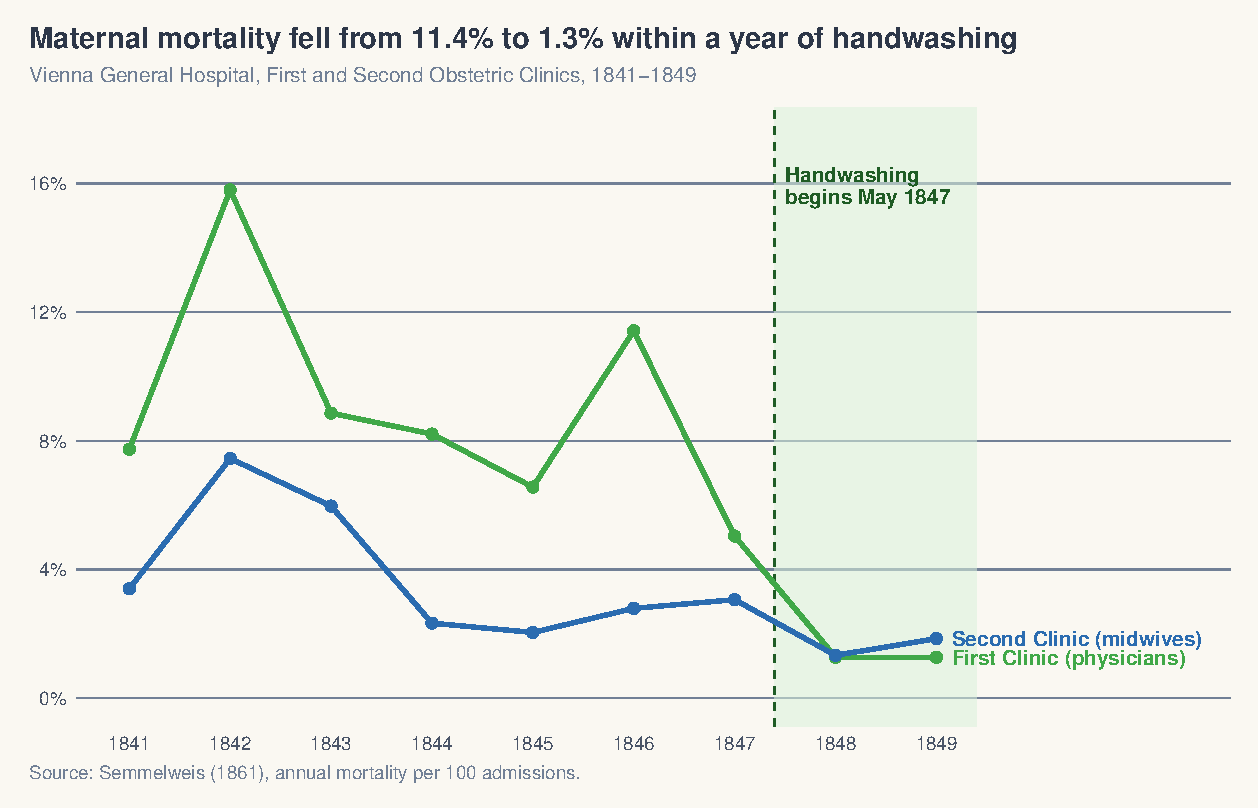
\includegraphics[height=0.72\textheight,keepaspectratio]{figures/semmelweis_remix.pdf}
\end{center}
\begin{center}
\small\color{warmgray}\itshape Monthly mortality, First Obstetric Clinic. Handwashing began mid-1847.
\end{center}
\end{frame}

%% --- 1.2 Princeton ---
\begin{frame}{Princeton, 1970s: Orley Ashenfelter}
\vspace{0.3em}
\footnotesize
The Industrial Relations Section was founded 1922 --- rigorous empirical labor research, the policy edge of US economics.
\vspace{0.3em}
\begin{block}{Orley Ashenfelter's leadership}
\begin{itemize}
  \item Long-time director. Set the tone: high-quality data, careful design, communicate to bureaucrats.
  \item Trained a cohort: \textbf{David Card}, \textbf{Josh Angrist}, \textbf{Bob LaLonde}, \textbf{Janet Currie}, Pischke, Dinardo, Case, others.
  \item Hired \textbf{Alan Krueger} as a junior colleague.
\end{itemize}
\end{block}
\end{frame}

%% --- 1.3 The late-1970s crisis + Orley video ---
\begin{frame}{By the late 1970s, empirical labor was in trouble}
\vspace{0.4em}
\begin{itemize}
  \item Different methods on the same question disagreed wildly
  \item The Princeton response: \highlight{design over modeling --- estimators that mimic an RCT as closely as possible}
  \item Worker surveys, federal job training, massive panel regressions
  \item Audience was bureaucrats
\end{itemize}
\vspace{0.6em}
\pullquote{Their eyes would glaze over whenever you said `regression.'}{Orley Ashenfelter}
\vspace{0.6em}
\begin{center}
\href{https://www.youtube.com/watch?v=WnB3EJ8K7lg\&t=14s}{\color{ocean}\underline{youtu.be/WnB3EJ8K7lg}} \;\small\color{warmgray}\itshape (3:53)
\end{center}
\end{frame}

%% ===========================================================
%% SECTION 2. DiD = calculation + assumption
%% ===========================================================
\remixsection{2.\ DiD is Two Things: a Calculation and an Assumption}

%% --- 2.1 Research design, not a regression ---
\begin{frame}{DiD is a research design, not a regression}
\vspace{1.0em}
\pullquote{A research design is an identification strategy: it reveals the invisible target parameter hidden inside a calculation.}{}
\vspace{1.0em}
\begin{center}
\begin{tikzpicture}
\node[ingredient] (calc) at (-3.2,0) {%
  \textcolor{accent}{\large 1.} \\[0.3em]
  A \textit{calculation}\\[0.2em]
  \scriptsize\textcolor{warmgray}{(the 2$\times$2)}
};
\node[ingredient] (assn) at (3.2,0) {%
  \textcolor{accent}{\large 2.} \\[0.3em]
  An \textit{assumption}\\[0.2em]
  \scriptsize\textcolor{warmgray}{(parallel trends)}
};
\node[font=\Large\bfseries,text=accent] at (0,0) {+};
\end{tikzpicture}
\end{center}
\end{frame}

%% --- 2.2 Individual treatment effect ---
\begin{frame}{The individual treatment effect}
\vspace{1.2em}
\begin{center}
\Large
\[
\delta_i \;=\; Y_i(1) - Y_i(0)
\]
\end{center}
\vspace{0.6em}
\begin{itemize}
  \item One per unit. \highlight{Different} across units in general --- treatment effects are heterogeneous.
  \item We only ever see one of $Y_i(1)$ or $Y_i(0)$. The other is the counterfactual.
  \item So $\delta_i$ is never directly observed at the individual level.
\end{itemize}
\end{frame}

%% --- 2.2b The ATT and the three ingredients of a causal parameter ---
\begin{frame}{The ATT: a causal parameter has three ingredients}
\vspace{1.4em}
\begin{center}
\Large
\[
\text{ATT} \;=\; \underbrace{\mathbb{E}\big[\,}_{\text{\normalsize \color{accent} weighted expectations}}\;
\underbrace{Y(1) - Y(0)}_{\text{\normalsize \color{accent} potential outcomes}}\;
\underbrace{\big|\; D = 1,\,\text{Post}\,\big]}_{\text{\normalsize \color{accent} population}}
\]
\end{center}
\vspace{1.4em}
\begin{itemize}
  \item \highlight{Potential outcomes} --- the contrast $Y(1) - Y(0)$
  \item \highlight{Population} --- on whom: treated units, post-period
  \item \highlight{Weighted expectations} --- how we average across that population ($\mathbb{E}[\cdot]$ defaults to equal weights)
\end{itemize}
\end{frame}

%% --- 2.3 Switching equation ---
\begin{frame}{The switching equation: you see one half}
\vspace{0.8em}
\begin{center}
\Large
\[
Y_i \;=\; D_i \cdot Y_i(1) \;+\; (1 - D_i) \cdot Y_i(0)
\]
\end{center}
\vspace{1em}
\begin{itemize}\setlength\itemsep{6pt}
  \item For each unit: $Y_i(1)$ if treated, $Y_i(0)$ if not.
  \item The ATT asks about \textit{both} columns. The data hands you one.
\end{itemize}
\vspace{0.8em}
\meta{The rest of the day: strategies for recovering the ATT from the half you see.}
\end{frame}

%% ===========================================================
%% SECTION 3. Five regressions, one number
%% ===========================================================
\remixsection{3.\ Five Regressions, One Number}

%% --- 3.1 Cheng & Hoekstra (2013) setup ---
\begin{frame}{Cheng \& Hoekstra (2013): castle doctrine and homicide}
\vspace{0.3em}
\footnotesize
\textbf{The reform.} ``Castle doctrine'' laws expanded the legal right to use lethal force in self-defense, removing the duty to retreat. Many US states passed expansions from \highlight{2005--2010}.
\vspace{0.4em}
\begin{itemize}
  \item \textbf{Panel:} all US states $\times$ years (state-year).
  \item \textbf{Outcome:} log homicide rate, FBI Supplementary Homicide Reports.
  \item \textbf{Treatment:} state passed an expansion of castle doctrine.
  \item \textbf{Comparison:} states that did not pass (never-treated).
\end{itemize}
\vspace{0.4em}
For today: a clean 2$\times$2 on \highlight{2005--2006}. Treated $=$ states adopting in 2006; control $=$ states that hadn't.
\vspace{0.4em}
\meta{Cheng \& Hoekstra (2013), ``Does Strengthening Self-Defense Law Deter Crime or Escalate Violence? Evidence from Expansions to Castle Doctrine.'' \textit{J. Human Resources} 48(3): 821--854.}
\end{frame}

%% --- 3.2 Four cells by hand on castle.dta ---
\begin{frame}[fragile]{The four cells, by hand on \texttt{castle.dta}}
\vspace{0.2em}
\begin{lstlisting}[language={[ANSI]C}]
use castle.dta, clear
keep if year >= 2005 & year <= 2006
gen post  = (year == 2006)
gen treat = (effyear == 2006)

summarize l_homicide if treat==1 & post==1   // Y11
summarize l_homicide if treat==1 & post==0   // Y10
summarize l_homicide if treat==0 & post==1   // Y01
summarize l_homicide if treat==0 & post==0   // Y00
\end{lstlisting}
\vspace{0.4em}
\begin{center}
\small
$\widehat{\text{DiD}} = (\overline{Y}_{11} - \overline{Y}_{10}) - (\overline{Y}_{01} - \overline{Y}_{00}) \;\approx\; \mathbf{0.10}$
\end{center}
\vspace{0.2em}
\begin{center}
\small\color{warmgray}\itshape Log homicide rate $\sim 10\%$ higher in 2006-adopting states relative to non-adopters.
\end{center}
\end{frame}

%% --- 3.3 Regression 1: OLS with interactions ---
\begin{frame}[fragile]{Regression 1: OLS with treat $\times$ post}
\vspace{0.4em}
\begin{lstlisting}[language={[ANSI]C}]
reg l_homicide post##treat, cluster(sid)
\end{lstlisting}
\vspace{0.8em}
The coefficient on \texttt{1.post\#1.treat} is the DiD.
\vspace{0.6em}
\begin{center}
$Y \;=\; \beta_0 + \beta_1\,\text{Post} + \beta_2\,\text{Treat} + \beta_3\,(\text{Post}\times\text{Treat}) + \varepsilon$
\end{center}
\vspace{0.4em}
\begin{center}
\small\color{warmgray}\itshape The saturated specification. $\hat\beta_3 \approx 0.10$.
\end{center}
\end{frame}

%% --- 3.4 Regression 2: TWFE ---
\begin{frame}[fragile]{Regression 2: two-way fixed effects}
\vspace{0.4em}
\begin{lstlisting}[language={[ANSI]C}]
xtset sid year
xtreg l_homicide c.treat#c.post i.year, fe vce(cluster sid)
\end{lstlisting}
\vspace{0.8em}
State fixed effects absorb time-invariant level differences. \;Year fixed effects absorb common shocks.
\vspace{0.4em}
\begin{center}
\small\color{warmgray}\itshape In the 2$\times$2 case, the TWFE coefficient equals the DiD. \;Same number.
\end{center}
\end{frame}

%% --- 3.5 Regression 3: First-difference on treatment dummy ---
\begin{frame}[fragile]{Regression 3: first-difference $\Delta Y_i$ on $D_i$}
\vspace{0.3em}
\begin{lstlisting}[language={[ANSI]C}]
keep sid year l_homicide treat
reshape wide l_homicide, i(sid) j(year)
gen dY = l_homicide2006 - l_homicide2005
reg dY treat, vce(cluster sid)
\end{lstlisting}
\vspace{0.6em}
\begin{center}
$\Delta Y_i \;=\; \alpha + \beta_{DD}\,D_i + u_i$
\end{center}
\vspace{0.4em}
\begin{itemize}\small
  \item Collapse the panel: one $\Delta Y$ per unit.
  \item Time-differencing wipes out unit fixed effects mechanically.
  \item Slope on \texttt{treat} = the DiD. \;Same number.
\end{itemize}
\end{frame}

%% --- 3.6 Regression 4: across-group difference on post dummy (NEW) ---
\begin{frame}[fragile]{Regression 4: $(Y_{\text{treat}} - Y_{\text{ctrl}})$ on the post dummy}
\vspace{0.3em}
At each time $t$, take the across-group difference $D_t = \overline{Y}_{1,t} - \overline{Y}_{0,t}$. Then regress on a post indicator:
\vspace{0.3em}
\begin{center}
$D_t \;=\; \alpha + \beta_{DD}\,\text{Post}_t + v_t$
\end{center}
\vspace{0.3em}
\begin{lstlisting}[language={[ANSI]C}]
collapse (mean) l_homicide, by(treat year)
reshape wide l_homicide, i(year) j(treat)
gen Dt   = l_homicide1 - l_homicide0
gen post = (year == 2006)
reg Dt post
\end{lstlisting}
\vspace{0.2em}
\begin{itemize}\small
  \item Regression 3 differences over \textit{time}; Regression 4 differences over \textit{groups} first.
  \item By Frisch--Waugh--Lovell, partialling out the two-way means runs in either order. \;Same number.
\end{itemize}
\end{frame}

%% --- 3.7 Regression 5: long differences / Snow-style two means ---
\begin{frame}{Regression 5: long differences --- the Snow move}
\vspace{0.6em}
Compute one number per group, post minus pre, then subtract:
\vspace{0.4em}
\begin{center}
\Large
\[
\widehat{\text{DiD}} \;=\; \big(\overline{Y}_{11} - \overline{Y}_{10}\big) \;-\; \big(\overline{Y}_{01} - \overline{Y}_{00}\big)
\]
\end{center}
\vspace{0.6em}
\begin{itemize}
  \item No regression. \;Two long differences. \;One subtraction between them.
  \item This is what John Snow did in 1854 with the water-company data.
  \item Identical to Regressions 1--4. \;\highlight{The arithmetic was the point all along.}
\end{itemize}
\end{frame}

%% --- 3.8 Five regressions, one number (summary) ---
\begin{frame}{Five regressions, one number}
\vspace{0.6em}
\begin{center}
\renewcommand{\arraystretch}{1.4}
\footnotesize
\begin{tabular}{@{}lcc@{}}
\toprule
\textbf{Specification} & \textbf{What it does} & \textbf{$\hat\beta_{DD}$} \\
\midrule
1.\ OLS with \texttt{post\#\#treat} & saturated interaction & \;\;\highlight{$\approx 0.10$} \\
2.\ Two-way fixed effects & absorb unit + time means & \;\;\highlight{$\approx 0.10$} \\
3.\ $\Delta Y_i$ on $D_i$ (first difference) & difference over time, then on $D$ & \;\;\highlight{$\approx 0.10$} \\
4.\ $D_t$ on $\text{Post}_t$ (across-group diff) & difference over groups, then on Post & \;\;\highlight{$\approx 0.10$} \\
5.\ Long differences (Snow) & two means, one subtraction & \;\;\highlight{$\approx 0.10$} \\
\bottomrule
\end{tabular}
\end{center}
\vspace{0.6em}
\begin{center}
\small\color{warmgray}\itshape
Same data, five specifications, identical to machine epsilon. \\ The 2$\times$2 is the object; the regressions are just five ways to ask for it.
\end{center}
\end{frame}

%% ===========================================================
%% SECTION 4. Decomposing the 2x2
%% ===========================================================
\remixsection{4.\ Decomposing the 2$\times$2}

%% --- 4.1 The proof: add a zero, rearrange ---
\begin{frame}{The proof: add a zero, rearrange (five steps)}
\vspace{-0.4em}
\footnotesize

\textbf{1.\ Start with the 2$\times$2:}
\vspace{-0.5em}
\[
\widehat{\text{DiD}} \;=\; \big[\mathbb{E}[Y\mid 1,\text{Post}] - \mathbb{E}[Y\mid 1,\text{Pre}]\big]
                    \;-\; \big[\mathbb{E}[Y\mid 0,\text{Post}] - \mathbb{E}[Y\mid 0,\text{Pre}]\big]
\]
\vspace{-1.0em}

\textbf{2.\ Switching equation.} Treated-post is $Y(1)$; the other three cells are $Y(0)$:
\vspace{-0.3em}
\[
\widehat{\text{DiD}} \;=\; \big[\mathbb{E}[Y(1)\mid 1,\text{Post}] - \mathbb{E}[Y(0)\mid 1,\text{Pre}]\big]
                    \;-\; \big[\mathbb{E}[Y(0)\mid 0,\text{Post}] - \mathbb{E}[Y(0)\mid 0,\text{Pre}]\big]
\]
\vspace{-0.4em}

\textbf{3.\ Add a zero.}\;Insert $+\,\mathbb{E}[Y(0)\mid 1,\text{Post}] - \mathbb{E}[Y(0)\mid 1,\text{Post}]$:
\vspace{-0.3em}
\begin{align*}
\widehat{\text{DiD}} \;=\;&
  \mathbb{E}[Y(1)\mid 1,\text{Post}] \;-\; \mathbb{E}[Y(0)\mid 1,\text{Post}] \\
& {} +\;\mathbb{E}[Y(0)\mid 1,\text{Post}] - \mathbb{E}[Y(0)\mid 1,\text{Pre}]
   \;-\; \big[\mathbb{E}[Y(0)\mid 0,\text{Post}] - \mathbb{E}[Y(0)\mid 0,\text{Pre}]\big]
\end{align*}
\vspace{-0.4em}

\textbf{4.\ Rearrange.}\;First two terms $=$ ATT; remainder $=$ difference in $Y(0)$ trends:
\vspace{-0.3em}
\[
\widehat{\text{DiD}} \;=\; \underbrace{\mathbb{E}[Y(1)-Y(0)\mid 1,\text{Post}]}_{\textstyle\text{\color{accent}\bfseries ATT}}
                    \;+\; \underbrace{\big\{\Delta\mathbb{E}[Y(0)\mid 1] \;-\; \Delta\mathbb{E}[Y(0)\mid 0]\big\}}_{\text{non-parallel-trends bias}}
\]
\vspace{-0.4em}

\textbf{5.\ Read.}\;If the bias equals zero (\textit{parallel trends}), then $\widehat{\text{DiD}} = \text{ATT}$.
\end{frame}

%% --- 4.2 The bias IS selection bias on trends ---
\begin{frame}{The bias term \textit{is} selection bias --- on trends, not levels}
\footnotesize
The ``non-parallel-trends bias'' isn't a new concept. It's selection bias, in a different costume.
\vspace{-0.5em}
\[
\text{bias} \;=\; \underbrace{\Delta\mathbb{E}[Y(0)\mid D{=}1]}_{\text{how treated's $Y(0)$ moves}} \;-\; \underbrace{\Delta\mathbb{E}[Y(0)\mid D{=}0]}_{\text{how controls' $Y(0)$ moves}}
\]
\vspace{-0.3em}
\begin{itemize}
  \item \textbf{Cross-section selection bias}: are treated and control different in \textit{levels} of $Y(0)$?
  \item \textbf{DiD's selection bias}: are treated and control different in \textit{trends} of $Y(0)$?
  \item Different levels are fine. Unit fixed effects soak them up.
  \item What can't differ is the \textit{rate} at which $Y(0)$ moves across groups.
\end{itemize}
\vspace{0.2em}
\begin{block}{The trade DiD makes vs.\ randomization}
RCTs: treated and controls identical in everything --- levels and trends. \\
DiD: identical only in \textit{trends} of $Y(0)$. \;\highlight{Cheaper assumption. Weaker identification.}
\end{block}
\end{frame}

%% --- 4.3 Case 1: NA holds ---
\begin{frame}{Case 1: NA holds, never-treated comparison}
\footnotesize
\textbf{Switching equation.} Treated-post is $Y(1)$; the other three cells are $Y(0)$.
\vspace{-0.2em}
\[
\widehat{\text{DiD}} \;=\; \big[\mathbb{E}[Y(1)|1,\text{Post}] - \mathbb{E}[Y(0)|1,\text{Pre}]\big]
                  \;-\; \big[\mathbb{E}[Y(0)|0,\text{Post}] - \mathbb{E}[Y(0)|0,\text{Pre}]\big]
\]
\vspace{-1.1em}

\textbf{Add the zero.} Insert $+\,\mathbb{E}[Y(0)|1,\text{Post}] - \mathbb{E}[Y(0)|1,\text{Post}]$. Rearrange:
\vspace{-0.3em}
\[
\widehat{\text{DiD}} \;=\; \underbrace{\mathbb{E}[Y(1)-Y(0)|1,\text{Post}]}_{\textstyle\text{\color{accent}\bfseries ATT}}
                  \;+\; \underbrace{\big\{\Delta\mathbb{E}[Y(0)|1] - \Delta\mathbb{E}[Y(0)|0]\big\}}_{\text{non-PT bias}\;=\;0\;\text{under PT}}
\]
\vspace{-0.6em}

\begin{block}{Numerical example}
ATT $= 10$, PT bias $= 0$. \quad $\widehat{\text{DiD}} = \mathbf{10}$. \;\checkmark
\end{block}
\end{frame}

%% --- 4.4 Case 2: NA fails (anticipation) ---
\begin{frame}{Case 2: NA fails --- anticipation contaminates $Y_{\text{Pre}}$}
\footnotesize
Suppose the treated group anticipates and adjusts \textit{before} the policy lands. Their pre-period outcome contains some $Y(1)$ response: \;$\mathbb{E}[Y|1,\text{Pre}] = \mathbb{E}[Y(0)|1,\text{Pre}] + \textcolor{accent}{\text{ATT}_{\text{pre}}}$.

\vspace{0.3em}
Same +0 trick, propagated:
\vspace{-0.3em}
\[
\widehat{\text{DiD}} \;=\; \underbrace{\text{ATT}_{\text{Post}}}_{\text{what we want}}
                  \;+\; \underbrace{\text{non-PT bias}}_{=\,0}
                  \;-\; \underbrace{\textcolor{accent}{\text{ATT}_{\text{pre}}}}_{\text{anticipation}}
\]
\vspace{-0.6em}

\begin{block}{Numerical example}
ATT $= 10$, PT bias $= 0$, ATT$_{\text{pre}} = 3$. \quad $\widehat{\text{DiD}} = 10 - 3 = \mathbf{7}$. \;\highlight{biased down}
\end{block}
\meta{If treatment effects are roughly constant, DiD can collapse to zero.}
\end{frame}

%% --- 4.5 Case 3: control group also treated ---
\begin{frame}{Case 3: the control group also receives treatment in Post}
\scriptsize
Now the comparison group's Post outcome is also $Y(1)$, not $Y(0)$. Switching equation:
\vspace{-0.3em}
\[
\widehat{\text{DiD}} \;=\; \big[\mathbb{E}[Y(1)|1,\text{Post}] - \mathbb{E}[Y(0)|1,\text{Pre}]\big] \;-\; \big[\mathbb{E}[Y(1)|0,\text{Post}] - \mathbb{E}[Y(0)|0,\text{Pre}]\big]
\]
\vspace{-1.0em}

\textbf{Add two zeros} --- one missing counterfactual on each side --- and rearrange:
\vspace{-0.2em}
\[
\widehat{\text{DiD}} \;=\; \underbrace{\mathbb{E}[Y(1){-}Y(0)|1,\text{Post}]}_{\textstyle\text{\color{accent}\bfseries ATT}}
   \;+\; \underbrace{\big\{\Delta\mathbb{E}[Y(0)|1] - \Delta\mathbb{E}[Y(0)|0]\big\}}_{\text{non-PT bias}\,=\,0\text{ under PT}}
   \;-\; \underbrace{\mathbb{E}[Y(1){-}Y(0)|0,\text{Post}]}_{\textstyle\text{\color{accent}\bfseries ATT}_{D{=}0,\text{Post}}\;\text{\rmfamily\itshape (spillover)}}
\]
\vspace{-0.4em}

\begin{block}{Numerical example}
ATT $= 10$, PT bias $= 0$, ATT$_{D{=}0,\text{Post}} = 4$. \quad $\widehat{\text{DiD}} = 10 - 4 = \mathbf{6}$. \;\highlight{biased toward zero}
\end{block}
\meta{Three cases, three failures of the punchline. The +0 trick still works --- only the zero you add changes.}
\end{frame}

%% --- 4.6 Summary: four ways the 2x2 decomposes ---
\begin{frame}{Summary: four ways the 2$\times$2 decomposes}
\vspace{0.4em}
\small
\renewcommand{\arraystretch}{1.5}
\begin{center}
\begin{tabular}{@{}p{0.50\textwidth}l@{}}
\toprule
\textbf{What holds} & $\widehat{\text{DiD}} \;=\;$ \\
\midrule
NA, never-treated control & ATT $+$ \textcolor{warmgray}{PT-bias} \\
PT, no NA, never-treated control & ATT$_{\text{Post}}$ $-$ \textcolor{warmgray}{ATT$_{\text{Pre}}$} \\
PT, NA, always-treated control & ATT $-$ \textcolor{warmgray}{$\Delta$ATT$_{D=0}$} \\
PT, NA, SUTVA fails (spillover) & ATT $-$ \textcolor{warmgray}{ATT$_{D=1,\text{Post}}$} \\
\bottomrule
\end{tabular}
\end{center}
\vspace{0.8em}
\meta{All four derivable the same way: write down the 2$\times$2, apply the switching equation, add the right series of zeros.}
\end{frame}

%% ===========================================================
%% SECTION 5. Card and Krueger
%% ===========================================================
\remixsection{5.\ Card and Krueger: Parallel Trends, Visualized}

%% --- 5.0a Parallel trends, drawn (moved here) ---
\begin{frame}{Parallel trends, drawn}
\vspace{0.2em}
\begin{center}
\begin{tikzpicture}[scale=0.92]
\draw[->, slate, thick] (0,0) -- (6.8,0) node[right, text=charcoal, font=\small] {time};
\draw[->, slate, thick] (0,0) -- (0,3.3) node[above, text=charcoal, font=\small] {$Y$};

\draw[dashed, warmgray] (2.5,0) -- (2.5,3.1);
\node[font=\scriptsize, text=warmgray, anchor=north] at (2.5,-0.1) {treatment};

\draw[trendcontrol] (0.3,0.6) -- (4.5,1.44);
\draw[trendline] (0.3,1.6) -- (2.5,2.04);
\draw[trendline] (2.5,2.04) -- (4.5,2.84);
\draw[line width=0.8pt, accent, densely dotted] (2.5,2.04) -- (4.5,2.44);

\draw[<->, accent, line width=0.5pt] (4.7,2.44) -- (4.7,2.84);
\node[font=\scriptsize, text=accent, anchor=west] at (4.78,2.64) {ATT};

\node[font=\scriptsize, text=slate,  anchor=west] at (5.3,1.44) {control $= Y(0)$};
\node[font=\scriptsize, text=accent, anchor=west] at (5.3,2.84) {treated $= Y(1)$};
\node[font=\scriptsize, text=accent, anchor=west] at (5.3,2.44) {$Y(0)$ counter.};
\end{tikzpicture}
\end{center}
\vspace{-0.2em}
\begin{center}
\footnotesize
$\mathbb{E}[Y(0)\mid D{=}1,\text{Post}] - \mathbb{E}[Y(0)\mid D{=}1,\text{Pre}] \;=\; \mathbb{E}[Y(0)\mid D{=}0,\text{Post}] - \mathbb{E}[Y(0)\mid D{=}0,\text{Pre}]$
\end{center}
\vspace{0.2em}
\begin{center}
\small\color{warmgray}\itshape
A 2$\times$2 of $Y(0)$ terms. \;\highlight{If it isn't four $Y(0)$s, it isn't the PTA.}
\end{center}
\end{frame}

%% --- 5.0b Under PT, the 2x2 hits the ATT (moved here) ---
\begin{frame}{Under PT, the 2$\times$2 hits the ATT}
\vspace{0.5em}
With (i) \highlight{No Anticipation}, (ii) \highlight{Parallel Trends in $Y(0)$}, and (iii) a clean (never-treated) comparison group:
\vspace{0.4em}
\begin{center}
\Large
\[
\text{ATT}_{\text{post}} \;=\; \underbrace{\mathbb{E}[\Delta Y \mid D=1]}_{\text{treated change}} \;-\; \underbrace{\mathbb{E}[\Delta Y \mid D=0]}_{\text{control change}}
\]
\end{center}
\vspace{0.4em}
\begin{itemize}\setlength\itemsep{4pt}
  \item The 2$\times$2 calculation equals the population's ATT.
  \item Four averages. Three subtractions. One target parameter.
\end{itemize}
\vspace{0.6em}
\begin{center}
\highlight{This is the punchline. Everything that follows is variations on this theme.}
\end{center}
\end{frame}

%% --- 5.1 NJ raises minimum wage ---
\begin{frame}{New Jersey raises its minimum wage. Pennsylvania doesn't.}
\vspace{0.4em}
\begin{itemize}
  \item \highlight{April 1992}: New Jersey raises its minimum wage from \$4.25 to \$5.05 --- a 19\% increase.
  \item Pennsylvania, just over the river, stays at \$4.25.
  \item Card and Krueger survey 410 fast-food restaurants on both sides of the border, before (Feb 1992) and after (Nov 1992).
  \item The natural 2$\times$2: \highlight{treated $=$ NJ, control $=$ PA, pre/post the policy.}
\end{itemize}
\vspace{0.4em}
\meta{Card \& Krueger, \textit{American Economic Review}, 1994.}
\end{frame}

%% --- 5.2 What Card and Krueger found ---
\begin{frame}{What Card and Krueger \textit{found}}
\vspace{0.4em}
\begin{center}
\renewcommand{\arraystretch}{1.4}
\footnotesize
\begin{tabular}{@{}lccc@{}}
\toprule
\textbf{Employment per restaurant} & \textbf{Pre (Feb 1992)} & \textbf{Post (Nov 1992)} & \textbf{Change} \\
\midrule
NJ (treated) & 20.44 & 21.03 & $+0.59$ \\
PA (control) & 23.33 & 21.17 & $-2.16$ \\
\midrule
\rowcolor{remixgreenlight}
\textbf{DiD (NJ -- PA)} & & & \highlight{\textbf{+2.76 jobs/restaurant}} \\
\bottomrule
\end{tabular}
\end{center}
\vspace{0.5em}
\begin{itemize}\small
  \item Employment in NJ fast food \textit{rose} slightly, relative to PA, after the wage hike.
  \item Standard error puts the effect roughly indistinguishable from zero --- but the sign is the opposite of what theory predicted.
  \item \highlight{No measurable disemployment effect.} The textbook had failed a real test.
\end{itemize}
\end{frame}

%% --- 5.3 Buchanan + Card combined ---
\begin{frame}{The reaction was personal}
\vspace{0.4em}
\pullquote{No self-respecting economist would claim that increases in the minimum wage increase employment. Such a claim becomes equivalent to a denial that there is even minimal scientific content in economics.}{James Buchanan (Nobel 1986), \textit{WSJ}, April 1996}
\vspace{0.4em}
\pullquote{It cost me a lot of friends. People that I had known for many years became very angry or disappointed. They thought that in publishing our work we were being traitors to the cause of economics as a whole.}{David Card, interview}
\vspace{0.2em}
\begin{center}
\small\color{warmgray}\itshape
The price of a credible empirical paper that contradicted the consensus. \;Krueger paid more.
\end{center}
\end{frame}

%% --- 5.3b Hear it from them: three short interview clips ---
\begin{frame}{Hear it from them --- three short interview clips}
\vspace{0.5em}
\begin{itemize}
  \item \textbf{Orley Ashenfelter on the profession's reaction} (start 31:20) \\
        \href{https://youtu.be/MOtbuRX4eyQ?t=1882}{\color{ocean}\texttt{youtu.be/MOtbuRX4eyQ?t=1882}}
  \vspace{0.3em}
  \item \textbf{Card on the hostility from peers} (1:07--1:10) \\
        \href{https://youtu.be/1soLdywFb_Q?si=laAVYf_E2KBZKywG&t=4020}{\color{ocean}\texttt{youtu.be/1soLdywFb\_Q?t=4020}}
  \vspace{0.3em}
  \item \textbf{Card on what happened to Alan Krueger} (1:16--1:17) \\
        \href{https://youtu.be/1soLdywFb_Q?si=jsb8h50ZosGDnKrv&t=4556}{\color{ocean}\texttt{youtu.be/1soLdywFb\_Q?t=4556}}
\end{itemize}
\vspace{0.6em}
\begin{center}
\small\color{warmgray}\itshape
The DiD literature did not arrive politely. \;It was earned through paper-by-paper combat, much of it personal.
\end{center}
\end{frame}

%% --- 5.4 PT visualized ---
\begin{frame}{Parallel trends visualized: the control \textit{is} the counterfactual}
\vspace{0.1em}
\begin{center}
\begin{tikzpicture}[scale=1.0]
\draw[->, slate, thick] (0,0) -- (7.0,0) node[right, text=charcoal, font=\small] {time};
\draw[->, slate, thick] (0,0) -- (0,3.3) node[above, text=charcoal, font=\small] {employment};

\draw[dashed, warmgray] (3.0,0) -- (3.0,3.0);
\node[font=\scriptsize, text=warmgray, anchor=north] at (3.0,-0.1) {April 1992};

\draw[trendcontrol] (0.5,2.2) -- (5.5,1.6);

\draw[trendline] (0.5,1.4) -- (3.0,1.1);

\draw[trendline] (3.0,1.1) -- (5.5,1.25);

\draw[line width=0.8pt, accent, densely dotted] (3.0,1.1) -- (5.5,0.8);

\draw[<->, accent, line width=0.5pt] (5.7,0.8) -- (5.7,1.25);
\node[font=\scriptsize, text=accent, anchor=west] at (5.78,1.025) {2$\times$2 = ATT};

\node[font=\scriptsize, text=slate,  anchor=west] at (5.65,1.6) {PA $= Y(0)$};
\node[font=\scriptsize, text=accent, anchor=west] at (5.65,1.25) {NJ observed};
\node[font=\scriptsize, text=accent, anchor=west] at (5.65,0.65) {NJ $Y(0)$ counter.};
\end{tikzpicture}
\end{center}
\vspace{0.1em}
\begin{center}
\small\color{warmgray}\itshape
The dotted line is what NJ would have done absent the policy. \;We never see it. \\
\highlight{PT lets PA's slope stand in for it.}
\end{center}
\end{frame}

%% --- 5.5 ASIDE slide: across-group PT ---
\begin{frame}{Aside: there's also an \textit{across-group} PT we never name}
\scriptsize
\begin{block}{The usual statement (within-group, across-time)}
The comparison group's $Y(0)$ trend stands in for what the treated group's $Y(0)$ trend would have been.
\end{block}
\begin{block}{The same assumption, stated from the other side (across-group, within-time)}
The treated group's $Y(0)$ trend (had they not been treated) would equal the comparison group's $Y(0)$ trend.
\end{block}
\begin{itemize}\setlength\itemsep{1pt}
  \item Two phrasings of one assumption: $Y(0)$ trends are common across groups.
  \item Event-study $\beta_k$ vs $t=-1$ computes the within-group across-time piece.
  \item Regression 3 ($\Delta Y$ on $D$) and Regression 4 ($D_t$ on Post) are FWL mirrors --- same PT from the two directions.
\end{itemize}
\meta{ASIDE --- drop in or drop out if behind schedule.}
\end{frame}

%% --- 5.6 Pre-trends are the gut check ---
\begin{frame}{Pre-trends are the gut check --- not a proof of PT}
\vspace{0.4em}
\begin{itemize}
  \item Card--Krueger held up because in the pre-period, NJ and PA fast-food employment moved together.
  \item If NJ employment had already been diverging before April 1992, the $+2.76$ estimate would have been mostly trend, not policy.
  \item Flat pre-trends $\rightarrow$ evidence (not proof) the design holds.
  \item \highlight{The 2$\times$2 was credible because of the pre-period parallelism --- not because of the regression coefficient.}
\end{itemize}
\vspace{0.4em}
\meta{More later (Roth, Roth--Sant'Anna): when pre-trends \textit{look} flat but the test still over-rejects.}
\end{frame}

%% ===========================================================
%% SECTION 6. Google Sheet
%% ===========================================================
\remixsection{6.\ Open the Sheet}

\begin{frame}{Open the Sheet: stability and trends, by hand}
\vspace{0.6em}
\begin{block}{Live demo}
Compute the four cells, three subtractions, and the by-hand event study --- in a spreadsheet.
\end{block}
\vspace{1em}
\begin{center}
\href{https://docs.google.com/spreadsheets/d/1onabpc14JdrGo6NFv0zCWo-nuWDLLV2L1qNogDT9SBw/edit?usp=sharing}{\color{ocean}\underline{\small\texttt{docs.google.com/spreadsheets/d/1onabpc14JdrGo6NFv0zCWo-nuWDLLV2L1qNogDT9SBw}}}
\end{center}
\vspace{1em}
\begin{center}
\small\color{warmgray}\itshape
Four tabs in sequence: \texttt{Potential Outcomes} $\rightarrow$ \texttt{2X2} $\rightarrow$ \texttt{Balancing} $\rightarrow$ \texttt{2XT \#1}.
\end{center}
\end{frame}

%% ===========================================================
%% SECTION 7. Standard errors
%% ===========================================================
\remixsection{7.\ Standard Errors}

%% --- 7.1 Three flavors ---
\begin{frame}{Three flavors of standard error}
\vspace{0.6em}
\begin{itemize}
  \item \highlight{Vanilla (homoskedastic)}: assumes $\text{Var}(\varepsilon_i \mid X_i) = \sigma^2$ for all $i$.
  \item \highlight{Robust (Eicker--Huber--White, HC)}: each residual speaks for itself --- handles heteroskedasticity.
  \item \highlight{Cluster-robust (CRVE)}: groups residuals by cluster; within-cluster errors correlate freely.
\end{itemize}
\vspace{0.6em}
\meta{Same point estimate, three different SEs. The SE you pick is a claim about the error structure.}
\end{frame}

%% --- 7.1b HC1 numerically — worked example with 6 obs ---
\begin{frame}[shrink=8]{HC1 numerically: each $\hat e_i^2$ weighted by leverage}
\vspace{0.2em}
\textbf{Six observations.}\; Three pairs at $\tilde x \in \{-2, 0, +2\}$.\; Fitted $\hat\beta_1 = 1$; residuals shown.
\vspace{0.5em}
\begin{center}
\renewcommand{\arraystretch}{1.15}
\footnotesize
\begin{tabular}{@{}cccrrr@{}}
\toprule
$i$ & cluster $g$ & $\tilde x_i$ & $\hat e_i$ & $\hat e_i^2$ & $\meat{\tilde x_i^2 \cdot \hat e_i^2}$ \\
\midrule
1 & 1 & $-2$ & $+0.5$ & $0.25$ & \meat{$1.00$} \\
2 & 1 & $-2$ & $+0.5$ & $0.25$ & \meat{$1.00$} \\
3 & 2 & $0$  & $-1.0$ & $1.00$ & \meat{$0.00$} \\
4 & 2 & $0$  & $-1.0$ & $1.00$ & \meat{$0.00$} \\
5 & 3 & $+2$ & $+0.5$ & $0.25$ & \meat{$1.00$} \\
6 & 3 & $+2$ & $+0.5$ & $0.25$ & \meat{$1.00$} \\
\midrule
\multicolumn{5}{r}{\meat{meat} $\;=\;$} & \meat{$\mathbf{4.00}$} \\
\bottomrule
\end{tabular}
\end{center}
\vspace{0.4em}

With $n=6$, $k=2$, and $S_{xx} = \sum_i \tilde x_i^2 = (-2)^2{+}(-2)^2{+}0{+}0{+}2^2{+}2^2 = \bread{16}$:
\[
\widehat{\text{Var}}_{\text{HC1}}(\hat\beta_1) \;=\; \tfrac{n}{n-k}\cdot \underbrace{\bread{\tfrac{1}{S_{xx}}}}_{\textstyle\bread{\text{bread}}}\cdot \underbrace{\meat{\text{meat}}}_{\textstyle \meat{4.00}} \cdot \underbrace{\bread{\tfrac{1}{S_{xx}}}}_{\textstyle\bread{\text{bread}}} \;=\; \tfrac{6}{4}\cdot \tfrac{\meat{4.00}}{\bread{16} \cdot \bread{16}} \;=\; \tfrac{6}{4}\cdot \tfrac{\meat{4.00}}{\bread{256}} \;=\; 0.02344
\]
\vspace{-0.4em}
\[
\;\;\Rightarrow\;\; \highlight{$\text{SE}_{\text{HC1}} = \sqrt{0.02344} \approx 0.153$}
\]
\vspace{0.0em}
\meta{Obs 3--4 contribute zero because $\tilde x = 0$ kills the leverage weight. \;\textbf{HC1 treats all 6 obs as independent.}}
\end{frame}

%% --- 7.2 Why HC barely helps in DiD ---
\begin{frame}{Why HC-robust barely helps in DiD}
\vspace{0.4em}
The HC correction reweights residuals by $X_i X_i'$. In a DiD with binary $D_i \in \{0,1\}$ and roughly balanced groups:
\vspace{0.4em}
\begin{itemize}
  \item Treated and control units have similar \textit{leverage}: each side carries $\approx$ half the weight in $X'X$.
  \item Residual variance is roughly symmetric across the two groups (binary $D$ doesn't generate a fan shape in $\hat e^2$).
  \item The weighted sum $\sum_i \hat e_i^2 X_i X_i'$ ends up not very different from $\hat\sigma^2(X'X)$.
\end{itemize}
\vspace{0.4em}
\begin{block}{Consequence}
\small
$\text{SE}_{\text{HC}} \approx \text{SE}_{\text{vanilla}}$ for typical DiD specifications. \\
\highlight{The over-rejection problem is not heteroskedasticity. It's something else.}
\end{block}
\end{frame}

%% --- 7.2b CRVE numerically — worked example with 6 obs ---
\begin{frame}[shrink=10]{CRVE numerically: same 6 obs, group scores, then square}
\vspace{0.2em}
\textbf{Same 6 observations.} Now compute $s_g = \sum_{i \in g} \tilde x_i \hat e_i$ for each cluster, then $s_g^2$:
\vspace{0.4em}
\begin{center}
\renewcommand{\arraystretch}{1.15}
\footnotesize
\begin{tabular}{@{}cccrr@{}}
\toprule
$i$ & $g$ & $\tilde x_i$ & $\hat e_i$ & $\tilde x_i \hat e_i$ \\
\midrule
1 & \textcolor{accent}{1} & $-2$ & $+0.5$ & \textcolor{accent}{$-1$} \\
2 & \textcolor{accent}{1} & $-2$ & $+0.5$ & \textcolor{accent}{$-1$} \\
3 & \textcolor{ocean}{2}  & $0$  & $-1.0$ & $0$ \\
4 & \textcolor{ocean}{2}  & $0$  & $-1.0$ & $0$ \\
5 & \textcolor{forest}{3} & $+2$ & $+0.5$ & \textcolor{forest}{$+1$} \\
6 & \textcolor{forest}{3} & $+2$ & $+0.5$ & \textcolor{forest}{$+1$} \\
\bottomrule
\end{tabular}
\hspace{1.0em}
\begin{tabular}{@{}crr@{}}
\toprule
$g$ & $s_g$ & $\meat{s_g^2}$ \\
\midrule
\textcolor{accent}{1}  & \textcolor{accent}{$-2$}  & \meat{$4$} \\
\textcolor{ocean}{2}   & $0$  & \meat{$0$} \\
\textcolor{forest}{3}  & \textcolor{forest}{$+2$} & \meat{$4$} \\
\midrule
\multicolumn{2}{r}{\meat{meat} $=$} & \meat{$\mathbf{8}$} \\
\bottomrule
\end{tabular}
\end{center}
\vspace{0.4em}

With $G=3$, $n=6$, $k=2$, and $S_{xx} = \sum_i \tilde x_i^2 = \bread{16}$, so $\bread{S_{xx}^2 = 256}$:
\[
\widehat{\text{Var}}_{\text{CRVE}}(\hat\beta_1) \;=\; \tfrac{G}{G-1}\cdot \tfrac{n-1}{n-k}\cdot \tfrac{\meat{\text{meat}}}{\bread{S_{xx}^2}} \;=\; \tfrac{3}{2}\cdot \tfrac{5}{4}\cdot \tfrac{\meat{8}}{\bread{256}} \;=\; 0.05859
\;\;\Rightarrow\;\; \highlight{$\text{SE}_{\text{CRVE}} \approx 0.242$}
\]
\begin{center}
\small\color{warmgray}\itshape
\textbf{HC1}: 0.153 \quad vs.\quad \textbf{CRVE}: 0.242 \quad (\highlight{58\% larger}). \;Same data. The cluster cross-terms changed the \meat{meat} from \meat{4} to \meat{8}.
\end{center}
\end{frame}

%% --- 7.3 BDM 2004 placebo ---
\begin{frame}{Bertrand, Duflo \& Mullainathan (QJE 2004): the placebo-law test}
\vspace{0.4em}
\textbf{``How Much Should We Trust Differences-in-Differences Estimates?''}
\vspace{0.4em}
\begin{itemize}\small
  \item BDM generate \textit{placebo laws}: assign random treatment dates to states in a real CPS panel.
  \item True effect by construction: $\beta = 0$. So $\Pr(\text{reject } H_0)$ should equal $\alpha = 5\%$.
  \item \textbf{Vanilla SE}: rejection rate $\approx \mathbf{45\%}$. Wildly over-rejects.
  \item \textbf{Heteroskedasticity-robust (HC1)}: rejection rate \textit{also} $\approx 45\%$. \highlight{HC barely moves the needle.}
  \item \textbf{Cluster-robust at state level}: rejection rate $\approx \mathbf{5\%}$. \;The fix.
\end{itemize}
\vspace{0.4em}
\begin{block}{Why HC doesn't save you}
\small
Binary, balanced $D$ + within-state serial correlation. \;The het-correction has nothing to do with the actual problem. \;\highlight{Clustering is doing all the work.}
\end{block}
\end{frame}

%% ===========================================================
%% SECTION 8. Population weighting
%% ===========================================================
\remixsection{8.\ Population Weighting}

%% --- 8.1 Ten people, two counties ---
\begin{frame}{Ten people, two counties}
\vspace{0.1em}
\begin{center}
\footnotesize
\renewcommand{\arraystretch}{1.05}
\begin{tabular}{@{}l c c c c@{}}
\toprule
\textbf{Person} & $Y(0)$ & $Y(1)$ & $\delta_i$ & \textbf{County} \\
\midrule
\rowcolor{remixgreenlight}Alan    & 0 & 1 &  1 & 1 \\
\rowcolor{remixgreenlight}Betty   & 1 & 1 &  0 & 1 \\
\rowcolor{remixgreenlight}Chad    & 1 & 1 &  0 & 1 \\
\rowcolor{remixgreenlight}Daniel  & 0 & 0 &  0 & 1 \\
\rowcolor{remixgreenlight}Edith   & 0 & 1 &  1 & 1 \\
\rowcolor{remixgreenlight}Frank   & 0 & 1 &  1 & 1 \\
\rowcolor{remixgreenlight}George  & 0 & 0 &  0 & 1 \\
\rowcolor{remixgreenlight}Hank    & 0 & 1 &  1 & 1 \\
\midrule
\rowcolor{oceanlight}Ida   & 1 & 0 & $-1$ & 2 \\
\rowcolor{oceanlight}Janet & 1 & 0 & $-1$ & 2 \\
\bottomrule
\end{tabular}
\end{center}
\vspace{0.3em}
\begin{center}
\small\color{warmgray}\itshape
County 1: eight people. \;County 2: two people. \;Compute the average $\delta$ for each county, and across all ten. Same answer?
\end{center}
\end{frame}

%% --- 8.2 Same data, two weights, two parameters ---
\begin{frame}{Same data, two weights, two parameters}
\vspace{0.6em}
\begin{itemize}
  \item \textbf{Within counties:} County 1 avg $\delta = \tfrac{1}{8}(1{+}0{+}0{+}0{+}1{+}1{+}0{+}1) = \mathbf{+0.5}$. \\
        \hspace{1.7em} County 2 avg $\delta = \tfrac{1}{2}(-1{+}(-1)) = \mathbf{-1.0}$.
  \item \textbf{ATE for the average person}: $\tfrac{1}{10}(8\cdot 0.5 + 2\cdot(-1)) = \mathbf{+0.2}$.
  \item \textbf{ATE for the average county}: $\tfrac{1}{2}(0.5 + (-1)) = \mathbf{-0.25}$.
\end{itemize}
\vspace{0.7em}
\begin{center}
\small\color{warmgray}\itshape Same potential outcomes. \highlight{Different signs.} \\ Whichever you report depends on what you're trying to answer.
\end{center}
\end{frame}

%% --- 8.3 Two parameters, two answers ---
\begin{frame}{Two parameters, two answers}
\vspace{0.4em}
\footnotesize
Scale the example up: \highlight{Texas, 254 counties, 30M people.} 5 biggest counties hold 41\% of the population. \;Half the population has $\delta_i \sim \mathcal{N}(+5, 1)$; half has $\delta_i \sim \mathcal{N}(-1, 0.5)$. So $\mathbb{E}[\delta] = +2$. Sort high-$\delta$ people into the 5 big counties.
\vspace{0.5em}
\begin{itemize}
  \item \textbf{Per-person ATE}: $\;\tfrac{1}{N}\sum_i \delta_i$ --- weight every person by $1/N$. \\
        15M high-$\delta$ balance 15M low-$\delta$. \;\highlight{Answer: $+2$.}
  \item \textbf{Avg of county ATEs}: $\tfrac{1}{254}\sum_c \overline{\delta}_c$ --- weight every county by $1/254$. \\
        $\tfrac{5(+5) + 249(-1)}{254} = \;\highlight{-0.88}$. \;The 249 small counties dominate.
\end{itemize}
\vspace{0.5em}
\begin{center}
\color{warmgray}\itshape
Same data. Two weights. Two parameters. \;Sometimes two signs.
\end{center}
\end{frame}

%% --- 8.3b Sorting on delta can flip the sign ---
\begin{frame}{Sorting on $\delta$ can flip the sign of your answer}
\begin{center}
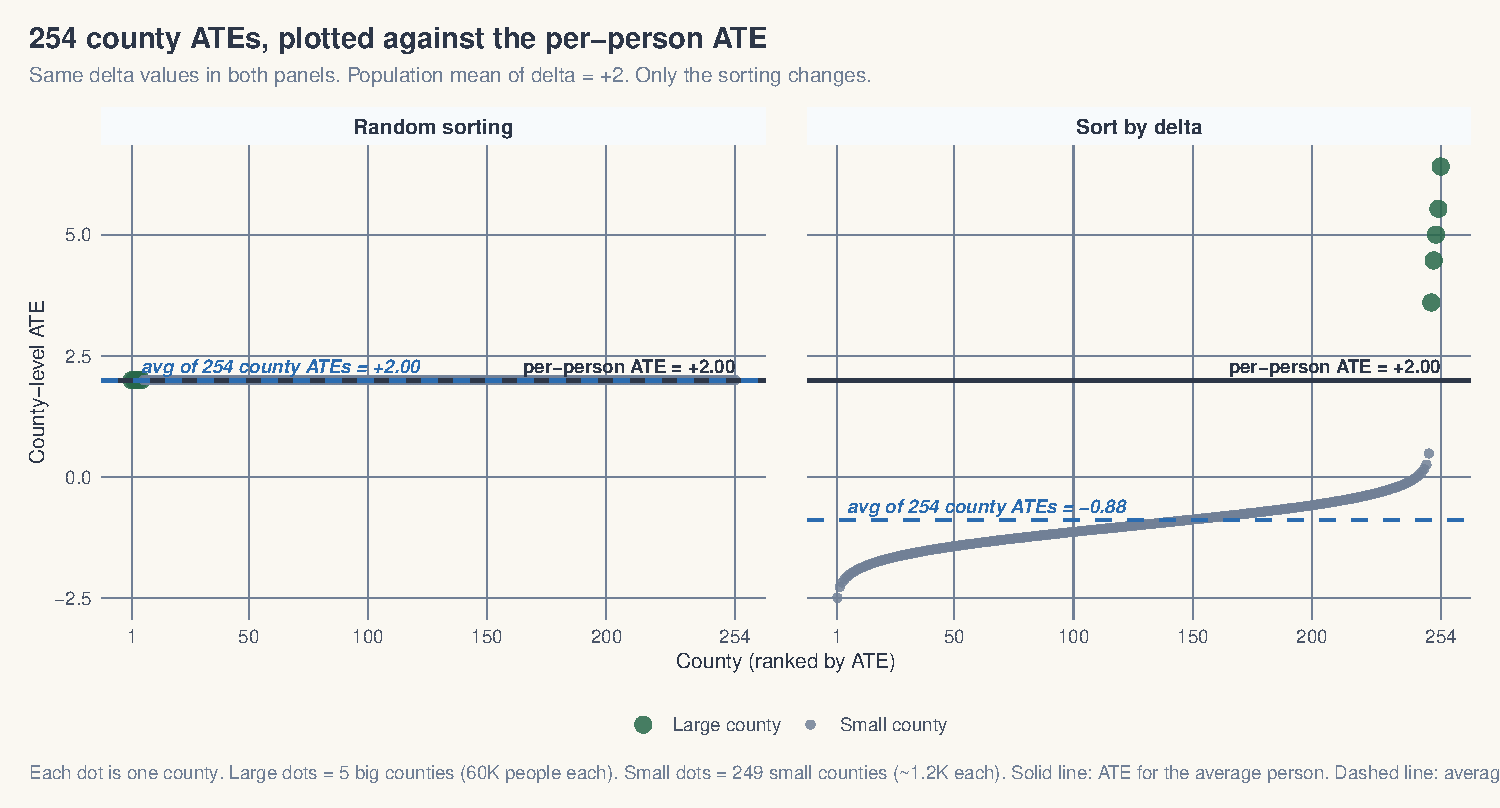
\includegraphics[width=0.92\linewidth,height=0.68\textheight,keepaspectratio]{figures/tiebout_roy_distributions.pdf}
\end{center}
\vspace{-0.3em}
\begin{center}
\scriptsize\color{warmgray}\itshape
Random: every county's ATE equals the population's. \;\;
$\delta$-sort: per-person line at $+2$, avg of county ATEs flips to \highlight{$-0.88$.} \\[0.15em]
Random sorting is the benchmark --- rarely reality. People choose where to live, and on traits that move $\delta$.
\end{center}
\end{frame}

%% --- 8.4 Pick a target parameter ---
\begin{frame}{Pick a target parameter}
\vspace{0.4em}
\begin{itemize}
  \item Three weights. \;Three signs. \;Three answers.
  \item The choice is about \textit{which causal effect you actually want}.
  \item \textbf{Person-weighted} for aggregate human welfare: how many people are affected, by how much?
  \item \textbf{Unit-weighted} when locations have autonomy: each policy unit chooses independently --- the unit \textit{is} the agent.
\end{itemize}
\vspace{0.8em}
\begin{center}
\Large\highlight{Today's target: the ATT.}
\end{center}
\vspace{0.4em}
\begin{center}
\small\color{warmgray}\itshape The average effect for the units that actually received the treatment.
\end{center}
\end{frame}

%% ===========================================================
%% SECTION 9. Event studies as falsification
%% ===========================================================
\remixsection{9.\ Event Studies: PT Made Falsifiable}

%% --- 9.0a What is a falsification? ---
\begin{frame}{Event studies are PT falsifications. What is a falsification?}
\vspace{0.6em}
\begin{itemize}\setlength\itemsep{0.5em}
  \item Popperian reasoning: \;you don't confirm a theory --- you try to falsify it.
  \item A rival theory earns scrutiny by making a \textit{prediction you can check}.
  \item Claim a confounder. Derive what \textit{else} it would do. Test that.
  \item If the prediction holds $\to$ you haven't confirmed the rival, but you haven't ruled it out either.
  \item If the prediction fails $\to$ the rival weakens.
\end{itemize}
\vspace{0.5em}
\meta{Popperian asymmetry. Failing to reject the rival does not confirm \textit{you}. But rejecting the rival's prediction is real evidence.}
\end{frame}

%% --- 9.0b Two forms of falsification ---
\begin{frame}{Two forms of falsification}
\vspace{0.6em}
\begin{itemize}\setlength\itemsep{0.7em}
  \item \highlight{Same outcome, different group.} A group your treatment shouldn't reach, but the rival would. \\
  \meta{Min wage on low-wage employment? Re-run on higher-wage workers.}
  \item \highlight{Same group, different outcome.} An outcome your treatment shouldn't move, but the rival would. \\
  \meta{Cigarette tax on smoking-related hospitalizations? Re-run on appendicitis and fractures.}
\end{itemize}
\vspace{0.6em}
\begin{center}
\small\color{warmgray}\itshape PT falsifications come in both forms. \;Event studies are one (same group, different ``outcome'' --- a period when no treatment happened).
\end{center}
\end{frame}

%% --- 9.0c Famous falsification 1: obesity contagion ---
\begin{frame}{Famous falsification 1: obesity contagion}
\vspace{0.6em}
\begin{itemize}\setlength\itemsep{0.5em}
  \item Christakis \& Fowler (2007): \;\textbf{obesity is contagious} in social networks.
  \item Cohen-Cole \& Fletcher (2008): \;re-run the same model on \highlight{height, acne, headaches} --- same Framingham network, same identification.
  \item All three also show ``contagion.''
\end{itemize}
\vspace{0.8em}
\pullquote{We have not been able to become taller by having tall friends.}{Cohen-Cole \& Fletcher (2008)}
\vspace{0.4em}
\meta{Same group, different outcome. \;The result isn't necessarily wrong --- the empirical model is.}
\end{frame}

%% --- 9.0d Famous falsification 2: milk addiction ---
\begin{frame}{Famous falsification 2: milk addiction}
\vspace{0.6em}
\begin{itemize}\setlength\itemsep{0.5em}
  \item Becker--Murphy (1988): \;serial correlation in cigarette / alcohol $\Rightarrow$ \textbf{``rational addiction.''}
  \item Auld \& Grootendorst (2004, \textit{J.\ Health Econ.}): \;apply the same estimator to \highlight{milk, eggs, oranges}.
  \item All three look ``rationally addictive.''
\end{itemize}
\vspace{0.8em}
\begin{center}
\small\color{warmgray}\itshape
Same group, different outcome. \;Nobody is rationally addicted to milk. \;\highlight{The identification --- not the goods --- is what's broken.}
\end{center}
\vspace{0.4em}
\meta{Point: \;PT makes predictions beyond the event study. \;Placebo groups and placebo outcomes are the other two forms.}
\end{frame}

%% --- 9.1 PT is about Y(0), not observed trends ---
\begin{frame}{Parallel trends is about $Y(0)$, not ``trends'' abstractly}
\footnotesize
The parallel-trends assumption is a statement about an unobserved object:
\vspace{-0.3em}
\[
\mathbb{E}\!\big[Y(0)_{t} - Y(0)_{t-1} \,\big|\, D{=}1\big] \;=\; \mathbb{E}\!\big[Y(0)_{t} - Y(0)_{t-1} \,\big|\, D{=}0\big]
\]
\vspace{-0.4em}
\begin{itemize}\setlength\itemsep{2pt}
  \item PT is the counterfactual untreated outcome's trend. \;\textbf{Not} a statement about OBSERVED $Y$ trends in general.
  \item Observed $Y$ for treated post-treatment is $Y(1)$, not $Y(0)$. \;The PT assumption can't be read off it.
  \item The confusion comes from saying ``trends are parallel.'' \;What we mean is ``\highlight{untreated potential outcome trends are parallel.}''
\end{itemize}
\begin{block}{Why this matters}
\scriptsize
We never see treated $Y(0)$ post-treatment. \;Pre-treatment data is the only window onto whether a similar assumption \textit{could} hold post. \;That's where event studies come in.
\end{block}
\end{frame}

%% --- 9.2 Why event studies — falsification of PT ---
\begin{frame}{Event studies: pre-treatment placebos for PT}
\vspace{0.2em}
\footnotesize
\textbf{The falsification logic.} \;Suppose some confounder both shifts $Y(0)$ trends \textit{and} is associated with treatment timing. \;That's a PT violation.

\vspace{0.4em}
\begin{itemize}\setlength\itemsep{3pt}
  \item If a similar confounder structure existed \textit{before} treatment, we should see treated and control $Y$ trends diverge in the pre-period too.
  \item Estimate placebo ``effects'' at $t=-2, -3, \ldots, -q$ where there is no treatment. If those coefficients are large or trending, we've rejected the assumption that drives the post-period.
\end{itemize}
\vspace{0.4em}
\begin{block}{Popperian asymmetry}
\small
Flat pre-trends \textit{fail to reject} PT --- they do not prove it. \\ Sloped pre-trends \textit{reject} the design.
\end{block}
\vspace{0.2em}
\begin{center}
\highlight{Pre-treatment placebos are a falsification, not a proof.}
\end{center}
\end{frame}

%% --- 9.3 Event study is 2x2 in motion ---
\begin{frame}{An event study is the 2$\times$2 viewed in motion}
\vspace{0.6em}
\begin{itemize}\setlength\itemsep{4pt}
  \item Instead of one pre-period and one post-period, use \textit{many}.
  \item Estimate a separate effect at each event-time relative to treatment.
  \item Plot them: $\hat{\beta}_{-q}, \ldots, \hat{\beta}_{-2}, \hat{\beta}_{-1}, \hat{\beta}_{0}, \hat{\beta}_{+1}, \ldots, \hat{\beta}_{+q}$.
  \item The graph tells two stories: \highlight{pre-trends} (left of zero) and \highlight{dynamics} (right of zero).
\end{itemize}
\vspace{0.4em}
\meta{Same arithmetic as the 2$\times$2, repeated against a common reference period.}
\end{frame}

%% --- 9.4 Every coefficient is a 2x2 against t = -1 ---
\begin{frame}{Every coefficient is a 2$\times$2 against $t = -1$}
\vspace{0.5em}
For each event-time $k$ (with $t = -1$ as the reference):
\vspace{-0.2em}
\[
\hat\beta_k \;=\; \big(\overline{Y}^T_k - \overline{Y}^T_{-1}\big) \;-\; \big(\overline{Y}^C_k - \overline{Y}^C_{-1}\big)
\]
\vspace{0.0em}
\begin{itemize}\setlength\itemsep{4pt}
  \item Two long differences, one subtraction --- the 2$\times$2 again, with $t=-1$ as the pre-period.
  \item Pre-period $\hat\beta_k$ ($k < -1$): asks whether trends were already diverging.
  \item Post-period $\hat\beta_k$ ($k \geq 0$): the dynamic ATTs.
\end{itemize}
\vspace{0.4em}
\meta{Drop $k = -1$ as the reference. Multicollinearity won't let you keep all the dummies.}
\end{frame}

%% --- 9.5 Saturated OLS specification ---
\begin{frame}{The saturated OLS specification}
\vspace{0.6em}
\begin{center}
\[
Y_{it} \;=\; \alpha_i \;+\; \tau_t \;+\; \sum_{t \neq t_0 - 1} \beta_t \cdot \big(D_i \cdot \mathbf{1}\{\text{year} = t\}\big) \;+\; \varepsilon_{it}
\]
\end{center}
\vspace{0.6em}
\begin{itemize}\setlength\itemsep{4pt}
  \item $\alpha_i$ --- unit fixed effects (absorb levels).
  \item $\tau_t$ --- calendar-year fixed effects (absorb common shocks).
  \item One interaction per calendar year, omitting $t_0 - 1$ (the year just before treatment) as the reference.
  \item Each $\beta_t$ is the 2$\times$2 of the previous slide: \;(treated change from $t_0{-}1$ to $t$) $-$ (control change from $t_0{-}1$ to $t$).
\end{itemize}
\vspace{0.4em}
\meta{In a 2$\times$T design the calendar year \textit{is} the event-time. We save $k$ for staggered treatment, where cohorts have different treatment dates.}
\end{frame}

%% --- 9.6 Tiny panel + by-hand calc (continues under §9) ---
\begin{frame}{A tiny panel where you can do the math in your head}
\footnotesize
\textbf{Cell means $\overline{Y}_{g,t}$.} Two treated units (T), two controls (C). Treatment turns on in 2000.
\vspace{0.4em}
\begin{center}
\renewcommand{\arraystretch}{1.2}
\begin{tabular}{@{}lccccc@{}}
\toprule
\textbf{Year $t$} & $1997$ & $1998$ & $1999$ & $2000$ & $2001$ \\
\midrule
\textbf{Treated} \;$\overline{Y}^T_t$ & $7$ & $8$ & $9$ & $13$ & $16$ \\
\textbf{Control} \;$\overline{Y}^C_t$ & $2$ & $3$ & $4$ & $5$ & $6$ \\
\midrule
$\overline{Y}^T_t - \overline{Y}^C_t$ & $5$ & $5$ & $5$ & $8$ & $10$ \\
\bottomrule
\end{tabular}
\end{center}
\vspace{0.5em}
\begin{itemize}\setlength\itemsep{2pt}
  \item Pre-period: T--C gap is constant at $5$. \;\highlight{Parallel trends.}
  \item True ATT$(2000) = 3$, True ATT$(2001) = 5$.
\end{itemize}
\end{frame}

%% --- 10.2 Each beta by hand, same via OLS ---
\begin{frame}[fragile]{Each $\hat\beta_t$ by hand --- same numbers via OLS}
\footnotesize
Formula: \;$\hat\beta_t \;=\; (\overline{Y}^T_t - \overline{Y}^T_{1999}) - (\overline{Y}^C_t - \overline{Y}^C_{1999})$
\vspace{0.4em}
\begin{columns}[T,onlytextwidth]
\column{0.50\textwidth}
\textbf{By hand}
\vspace{0.2em}
\begin{center}
\renewcommand{\arraystretch}{1.3}
\begin{tabular}{@{}lll@{}}
\toprule
$t$ & Calculation & $\hat\beta_t$ \\
\midrule
$1997$ & $(7{-}9) - (2{-}4)$ & $\mathbf{0}$ \\
$1998$ & $(8{-}9) - (3{-}4)$ & $\mathbf{0}$ \\
$2000$ & $(13{-}9) - (5{-}4)$ & $\mathbf{3}$ \\
$2001$ & $(16{-}9) - (6{-}4)$ & $\mathbf{5}$ \\
\bottomrule
\end{tabular}
\end{center}
\column{0.50\textwidth}
\textbf{Via OLS in R}
\begin{lstlisting}[language=R,basicstyle=\ttfamily\scriptsize]
library(fixest)
feols(Y ~ i(year, treat,
            ref = 1999) | unit + year,
      data = toy)
\end{lstlisting}
\vspace{0.2em}
\begin{center}
\renewcommand{\arraystretch}{1.15}
\scriptsize
\begin{tabular}{@{}lc@{}}
\toprule
coefficient & estimate \\
\midrule
\texttt{year::1997:treat} & $0$ \\
\texttt{year::1998:treat} & $0$ \\
\texttt{year::2000:treat} & $3$ \\
\texttt{year::2001:treat} & $5$ \\
\bottomrule
\end{tabular}
\end{center}
\end{columns}
\vspace{0.4em}
\begin{center}
\small\color{warmgray}\itshape OLS matches the manual 2$\times$2s to machine epsilon. \;The regression \textit{is} the formula.
\end{center}
\end{frame}

%% ===========================================================
%% SECTION 12. Closing: five pieces
%% ===========================================================
\remixsection{10.\ Five Pieces of a Strong DiD}

%% --- 12.1 The five pieces ---
\begin{frame}{Five pieces of a strong DiD}
\vspace{0.6em}
\begin{enumerate}
  \item \textbf{\color{accent}Bite} --- the policy actually changed what it was supposed to change.
  \item \textbf{\color{accent}Event study} --- pre/post coefficients around treatment.
  \item \textbf{\color{accent}Falsification} --- run a rival theory on a placebo group or outcome and try to reject \textit{it}.
  \item \textbf{\color{accent}Main result} --- the DiD on the actual outcome.
  \item \textbf{\color{accent}Mechanism} --- the causal pathway from $D$ to $Y$.
\end{enumerate}
\vspace{0.6em}
\meta{The point estimate alone is a case so weak that readers and the public are justified to reject it.}
\end{frame}

%% --- 12.2 Bite #1 ---
\begin{frame}{Bite \#1: Medicaid take-up jumped in expansion states}
\begin{center}
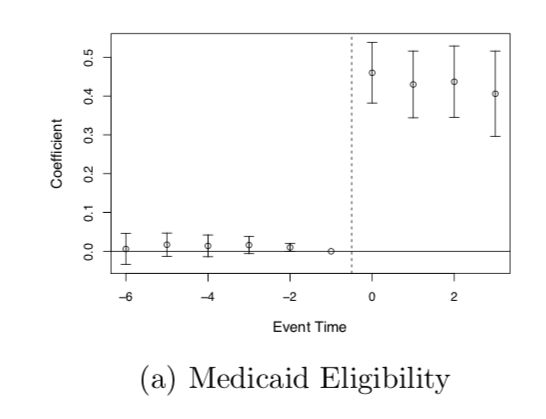
\includegraphics[height=0.60\textheight,keepaspectratio]{figures/Miller_Medicaid1.png}
\end{center}
\vspace{-0.2em}
\begin{center}
\footnotesize\color{warmgray}\itshape
\highlight{Did the policy actually move people onto Medicaid?}\; Yes --- enrollment rose sharply in expansion states post-2014, flat in non-expansion. \\
Without bite, there's no story. The mandate has to actually \textit{do} something before we can attribute downstream changes to it.
\end{center}
\end{frame}

%% --- 12.3 Bite #2 ---
\begin{frame}{Bite \#2: any-insurance coverage rose}
\begin{center}
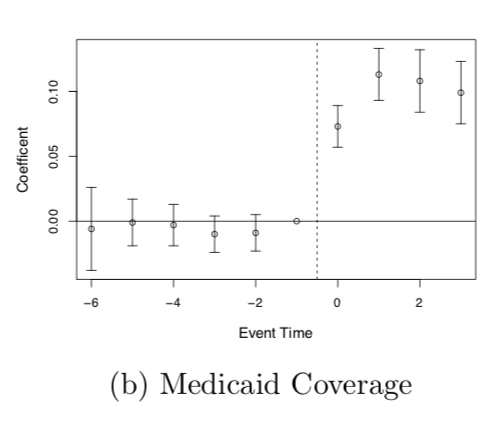
\includegraphics[height=0.62\textheight,keepaspectratio]{figures/Miller_Medicaid2.png}
\end{center}
\vspace{-0.2em}
\begin{center}
\footnotesize\color{warmgray}\itshape
\highlight{Did the new Medicaid enrollees actually gain coverage they didn't have?}\; Or did they just shift from private to Medicaid? \\
Any-insurance coverage rose --- the expansion brought in the previously uninsured, not the already-insured.
\end{center}
\end{frame}

%% --- 12.4 Bite #3 ---
\begin{frame}{Bite \#3: the uninsured rate fell}
\begin{center}
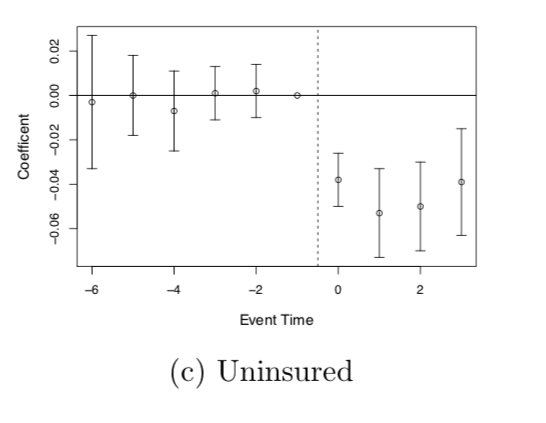
\includegraphics[height=0.62\textheight,keepaspectratio]{figures/Miller_Medicaid3.png}
\end{center}
\vspace{-0.2em}
\begin{center}
\footnotesize\color{warmgray}\itshape
\highlight{The mirror image of Bite \#2.}\; Uninsured rate dropped sharply in expansion states post-2014. \\
Three measures (Medicaid up, any-insurance up, uninsured down) converge on the same conclusion: \highlight{the policy bit.}
\end{center}
\end{frame}

%% --- 12.5 Falsification on 65+ ---
\begin{frame}{Falsification: same model, on the 65+ population --- no effect}
\begin{center}
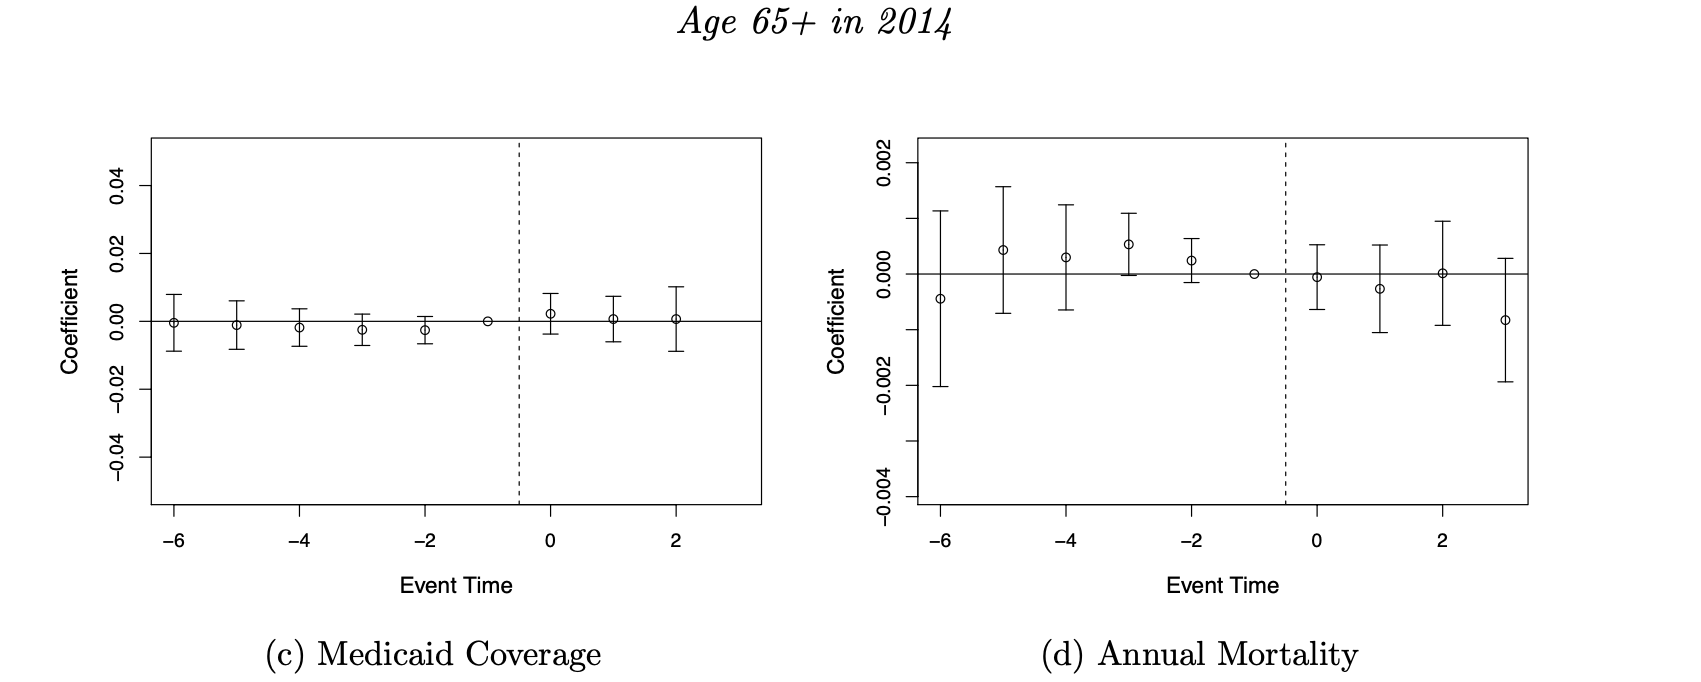
\includegraphics[height=0.60\textheight,keepaspectratio]{figures/placebo_medicaid.png}
\end{center}
\vspace{-0.2em}
\begin{center}
\footnotesize\color{warmgray}\itshape
\highlight{Same states, same years, same model --- but run on the 65+ population.}\; They all have Medicare, so Medicaid expansion shouldn't touch their mortality. \\
A rival theory (``some 2014 shock hit expansion states'') would predict a mortality effect here. It didn't appear. \highlight{Rival rejected.}
\end{center}
\end{frame}

%% --- 12.6 Medicaid main result ---
\begin{frame}{Medicaid expansion: $\approx 9.2\%$ reduction in near-elderly mortality}
\vspace{0.4em}
\textbf{Miller, Johnson \& Wherry (2021),} \textit{Quarterly Journal of Economics}.
\vspace{0.4em}
\begin{itemize}\small
  \item Did the ACA Medicaid expansion (2014) reduce mortality among the \highlight{near-elderly} (55--64)?
  \item Comparison: states that expanded vs.\ states that didn't, before vs.\ after 2014.
  \item Pre-trends flat. Post-2014 mortality declines in expansion states.
  \item Effect grows over time --- consistent with cumulative treatment for chronic conditions.
\end{itemize}
\vspace{0.5em}
\begin{block}{Why \textit{near}-elderly?}
\small
Everyone 65$+$ has Medicare --- Medicaid expansion is irrelevant for them. \;The elderly become a natural \highlight{placebo group} living in the same economies.
\end{block}
\end{frame}

%% --- 12.3 All five present ---
\begin{frame}{The five pieces, all five present in Medicaid}
\vspace{0.4em}
\begin{center}
\renewcommand{\arraystretch}{1.45}
\footnotesize
\begin{tabular}{@{}p{0.18\textwidth} p{0.74\textwidth}@{}}
\toprule
\textbf{Bite} & Three figures: Medicaid take-up up, any-insurance up, uninsured down \\
\textbf{Event study} & Pre-trends flat; post-trends decline in expansion states \\
\textbf{Falsification} & No effect on elderly (65+) --- same states, same years, same model \\
\textbf{Main result} & $\approx 9.2\%$ reduction in mortality among the near-elderly \\
\textbf{Mechanism} & Disease-related deaths fall and compound; consistent with treated chronic conditions \\
\bottomrule
\end{tabular}
\end{center}
\vspace{0.6em}
\begin{center}
\small\color{warmgray}\itshape
None of these alone is the case. \;\highlight{Together they are powerful.}
\end{center}
\end{frame}

%% --- 12.4 What we've done today + tomorrow ---
\begin{frame}{What we've done today --- and tomorrow}
\vspace{0.3em}
\textbf{Today:}
\begin{enumerate}\small
  \item DiD's empirical roots --- Semmelweis, Ashenfelter.
  \item DiD $=$ calculation $+$ assumption: the 2$\times$2 and parallel trends.
  \item Five regressions, one number.
  \item Decomposing the 2$\times$2 --- the +0 trick and three failure cases.
  \item Card and Krueger: parallel trends visualized.
  \item Standard errors --- vanilla, robust, cluster.
  \item Population weighting: pick a target parameter.
  \item Event studies as falsifications, by hand and via OLS.
\end{enumerate}
\vspace{0.5em}
\textbf{Tomorrow:} when the 2$\times$2 stops working --- covariates, staggered adoption (Goodman-Bacon, Callaway--Sant'Anna, Sun--Abraham, BJS, dCdH).
\end{frame}

\end{document}
